\documentclass{ximera}

\input{../../preamble.tex}

\title{Examples of Surjective Linear Transformations}

\begin{document}
\begin{abstract}
  We consider examples of surjective linear transformations, as well as examples which are not surjective.
\end{abstract}
\maketitle

It is perhaps most instructive to examine a linear transformation that is not surjective first.

\begin{example}[Not surjective]
Consider
\[\ltdefn{T}{\complex{5}}{\complex{5}},\quad
\lteval{T}{\colvector{x_1\\x_2\\x_3\\x_4\\x_5}}=
\colvector{-2 x_1 + 3 x_2 + 3 x_3 - 6 x_4 + 3 x_5\\
-16 x_1 + 9 x_2 + 12 x_3 - 28 x_4 + 28 x_5\\
-19 x_1 + 7 x_2 + 14 x_3 - 32 x_4 + 37 x_5\\
-21 x_1 + 9 x_2 + 15 x_3 - 35 x_4 + 39 x_5\\
-9 x_1 + 5 x_2 + 7 x_3 - 16 x_4 + 16 x_5}
\]

We will demonstrate that
\[
\vect{v}=\colvector{-1\\2\\3\\-1\\4}
\]
is an unobtainable element of the codomain.  Suppose to the contrary that $\vect{u}$ is an element of the domain such that $\lteval{T}{\vect{u}}=\vect{v}$.

Then
\begin{align*}
\colvector{-1\\2\\3\\-1\\4}&=\vect{v}=\lteval{T}{\vect{u}}
=\lteval{T}{\colvector{u_1\\u_2\\u_3\\u_4\\u_5}}\\
&=\colvector{
-2 u_1 + 3 u_2 + 3 u_3 - 6 u_4 + 3 u_5\\
-16 u_1 + 9 u_2 + 12 u_3 - 28 u_4 + 28 u_5\\
-19 u_1 + 7 u_2 + 14 u_3 - 32 u_4 + 37 u_5\\
-21 u_1 + 9 u_2 + 15 u_3 - 35 u_4 + 39 u_5\\
-9 u_1 + 5 u_2 + 7 u_3 - 16 u_4 + 16 u_5}\\
&=
\begin{bmatrix}
-2&3&3&-6&3\\
-16&9&12&-28&28\\
-19&7&14&-32&37\\
-21&9&15&-35&39\\
-9&5&7&-16&16
\end{bmatrix}
\colvector{u_1\\u_2\\u_3\\u_4\\u_5}
\end{align*}

Now we recognize the appropriate input vector $\vect{u}$ as a solution to a linear system of equations.  Form the augmented matrix of the system, and row-reduce to
\[
\begin{bmatrix}
\leading{1} & 0 & 0 & 0 & -1 & 0\\
0 & \leading{1} & 0 & 0 & -\frac{4}{3} & 0\\
0 & 0 & \leading{1} & 0 & -\frac{1}{3} & 0\\
0 & 0 & 0 & \leading{1} & -1 & 0\\
0 & 0 & 0 & 0 & 0 & \leading{1}\\
\end{bmatrix}
\]


With a leading 1 in the \wordChoice{\choice{first}\choice[correct]{last}} column, \ref{theorem:RCLS} tells us the system is \wordChoice{\choice{consistent}\choice[correct]{inconsistent}}.  From the absence of any solutions we conclude that no such vector $\vect{u}$ exists, and by \ref{definition:SLT}, $T$ is not surjective.

Again, do not concern yourself with how $\vect{v}$ was selected, as this will be explained shortly.  However, do understand \textit{why} this vector provides enough evidence to conclude that $T$ is not surjective.

\end{example}

Here is a cartoon of a non-surjective linear transformation.  Notice that the central feature of this cartoon is that the vector $\vect{v}\in V$ does not have an arrow pointing to it, implying there is no $\vect{u}\in U$ such that $\lteval{T}{\vect{u}}=\vect{v}$.  Even though this happens again with a second unnamed vector in $V$, it only takes one occurrence to destroy the possibility of surjectivity.
\begin{image}
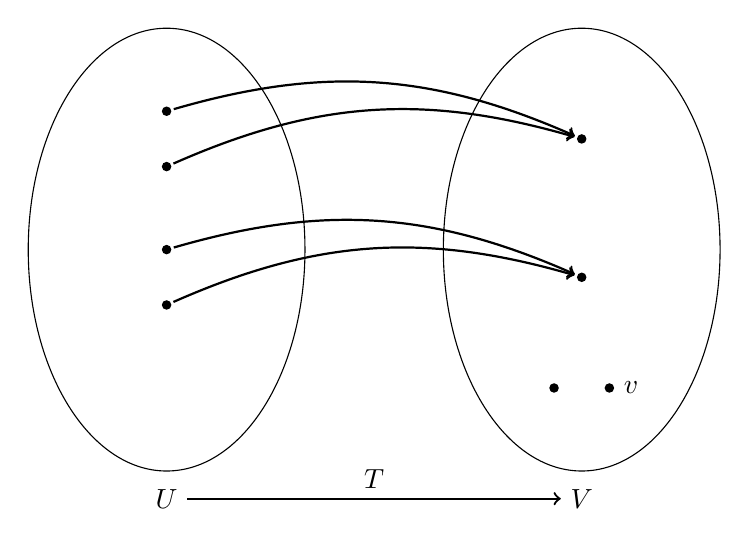
\begin{tikzpicture}
\tikzset{ltvect/.style={shape=circle, minimum size=0.30em, inner sep=0pt, draw, fill=black}}
\tikzset{ltedge/.style={->, bend left=20, thick, shorten <=0.1em, shorten >=0.1em}}
% base generic picture
\draw ( 5em, 8em) circle [x radius=5em, y radius=8em, thick];
\draw (20em, 8em) circle [x radius=5em, y radius=8em, thick];
\node (U) at ( 5em, -1em) {$U$};
\node (V) at (20em, -1em) {$V$};
\draw[->, thick, draw] (U) to node[auto] {$T$} (V);
% inputs
\node (u1) [ltvect]                         at (5em, 13em) {};
\node (u2) [ltvect]                         at (5em, 11em) {};
\node (u3) [ltvect]                         at (5em,  8em) {};
\node (u4) [ltvect]                         at (5em,  6em) {};
% outputs
\node (v1) [ltvect]                         at (20em, 12em) {};
\node (v2) [ltvect]                         at (20em,  7em) {};
\node (v3) [ltvect]                         at (19em,  3em) {};
\node (v)  [ltvect, label=right:$\vect{v}$] at (21em,  3em) {};
% associations
\draw[ltedge] (u1) to (v1);
\draw[ltedge] (u2) to (v1);
\draw[ltedge] (u3) to (v2);
\draw[ltedge] (u4) to (v2);
\end{tikzpicture}
\end{image}

To show that a linear transformation is not surjective, it is enough to find a single element of the codomain that is never created by any input, as in \ref{example:NSAQ}.  However, to show that a linear transformation is surjective we must establish that \textit{every} element of the codomain occurs as an output of the linear transformation for some appropriate input.


\begin{example}

Consider the linear transformation
\[
\ltdefn{T}{\complex{5}}{\complex{5}},\quad
\lteval{T}{\colvector{x_1\\x_2\\x_3\\x_4\\x_5}}=
\colvector{-65 x_1 + 128 x_2 + 10 x_3 - 262 x_4 + 40 x_5\\
36 x_1 - 73 x_2 - x_3 + 151 x_4 - 16 x_5\\
-44 x_1 + 88 x_2 + 5 x_3 - 180 x_4 + 24 x_5\\
34 x_1 - 68 x_2 - 3 x_3 + 140 x_4 - 18 x_5\\
12 x_1 - 24 x_2 - x_3 + 49 x_4 - 5 x_5}
\]


To establish that this transformation is surjective we must begin with a totally arbitrary element of the codomain, $\vect{v}$ and somehow find an input vector $\vect{u}$ such that $\lteval{T}{\vect{u}}=\vect{v}$.  We desire,
\begin{align*}
\lteval{T}{\vect{u}}&=\vect{v}\\
\colvector{-65 u_1 + 128 u_2 + 10 u_3 - 262 u_4 + 40 u_5\\
36 u_1 - 73 u_2 - u_3 + 151 u_4 - 16 u_5\\
-44 u_1 + 88 u_2 + 5 u_3 - 180 u_4 + 24 u_5\\
34 u_1 - 68 u_2 - 3 u_3 + 140 u_4 - 18 u_5\\
12 u_1 - 24 u_2 - u_3 + 49 u_4 - 5 u_5}
&=
\colvector{v_1\\v_2\\v_3\\v_4\\v_5}\\
\begin{bmatrix}
-65&128&10&-262&40\\
36&-73&-1&151&-16\\
-44&88&5&-180&24\\
34&-68&-3&140&-18\\
12&-24&-1&49&-5
\end{bmatrix}
\colvector{u_1\\u_2\\u_3\\u_4\\u_5}
&=
\colvector{v_1\\v_2\\v_3\\v_4\\v_5}
\end{align*}




We recognize this equation as a system of equations in the variables $u_i$, but our vector of constants contains symbols.  In general, we would have to row-reduce the augmented matrix by hand, due to the symbolic final column.  However, in this particular example, the $5\times 5$ coefficient matrix is nonsingular and so has an inverse (\ref{theorem:NI}, \ref{definition:MI}).
\[
\inverse{
\begin{bmatrix}
-65&128&10&-262&40\\
36&-73&-1&151&-16\\
-44&88&5&-180&24\\
34&-68&-3&140&-18\\
12&-24&-1&49&-5
\end{bmatrix}
}
=
\begin{bmatrix}
-47 & 92 &  1 & -181 & -14 \\
 27 & -55 & \frac{7}{2} & \frac{221}{2} & 11\\
-32 & 64  & -1 &  -126 &  -12\\
 25 &  -50 &  \frac{3}{2} & \frac{199}{2} & 9 \\
 9 & -18 & \frac{1}{2} & \frac{71}{2} & 4
\end{bmatrix}
\]
so we find that
\begin{align*}
\colvector{u_1\\u_2\\u_3\\u_4\\u_5}
&=
\begin{bmatrix}
-47 & 92 &  1 & -181 & -14 \\
 27 & -55 & \frac{7}{2} & \frac{221}{2} & 11\\
-32 & 64  & -1 &  -126 &  -12\\
 25 &  -50 &  \frac{3}{2} & \frac{199}{2} & 9 \\
 9 & -18 & \frac{1}{2} & \frac{71}{2} & 4
\end{bmatrix}
\colvector{v_1\\v_2\\v_3\\v_4\\v_5}\\
&=
\colvector{-47 v_1 + 92 v_2 + v_3 - 181 v_4 - 14 v_5\\
 27 v_1 - 55 v_2 + \frac{7}{2} v_3 + \frac{221}{2} v_4  + 11 v_5\\
-32 v_1 + 64  v_2 - v_3 - 126 v_4 - 12 v_5\\
 25 v_1 - 50 v_2 + \frac{3}{2} v_3 + \frac{199}{2} v_4 + 9 v_5\\
 9 v_1 - 18 v_2 + \frac{1}{2} v_3 + \frac{71}{2} v_4 + 4 v_5}
\end{align*}


This establishes that if we are given \textit{any} output vector $\vect{v}$, we can use its components in this final expression to formulate a vector $\vect{u}$ such that $\lteval{T}{\vect{u}}=\vect{v}$.  So by \ref{definition:SLT} we now know that $T$ is surjective.  You might try to verify this condition in its full generality (i.e.,  evaluate $T$ with this final expression and see if you get $\vect{v}$ as the result), or test it more specifically for some numerical vector $\vect{v}$.

\end{example}

Here is the cartoon for a surjective linear transformation.  It is meant to suggest that for every output in $V$ there is <em>at least one</em> input in $U$ that is sent to the output.  (Even though we have depicted several inputs sent to each output.)  The key feature of this cartoon is that there are no vectors in $V$ without an arrow pointing to them.
\begin{image}
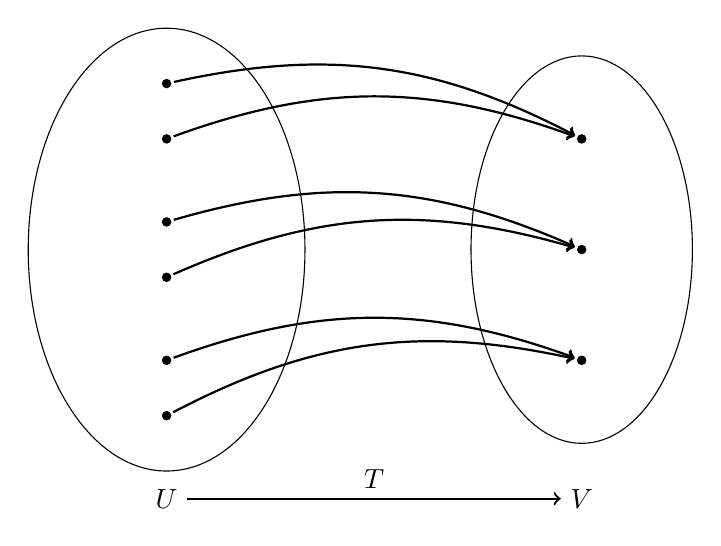
\begin{tikzpicture}
\tikzset{ltvect/.style={shape=circle, minimum size=0.30em, inner sep=0pt, draw, fill=black}}
\tikzset{ltedge/.style={->, bend left=20, thick, shorten <=0.1em, shorten >=0.1em}}
% base generic picture
\draw ( 5em, 8em) circle [x radius=5em, y radius=8em, thick];
\draw (20em, 8em) circle [x radius=4em, y radius=7em, thick];
\node (U) at ( 5em, -1em) {$U$};
\node (V) at (20em, -1em) {$V$};
\draw[->, thick, draw] (U) to node[auto] {$T$} (V);
% inputs
\node (u1) [ltvect]                         at (5em, 14em) {};
\node (u2) [ltvect]                         at (5em, 12em) {};
\node (u3) [ltvect]                         at (5em,  9em) {};
\node (u4) [ltvect]                         at (5em,  7em) {};
\node (u5) [ltvect]                         at (5em,  4em) {};
\node (u6) [ltvect]                         at (5em,  2em) {};
% outputs
\node (v1) [ltvect]                         at (20em, 12em) {};
\node (v2) [ltvect]                         at (20em,  8em) {};
\node (v3) [ltvect]                         at (20em,  4em) {};
% associations
\draw[ltedge] (u1) to (v1);
\draw[ltedge] (u2) to (v1);
\draw[ltedge] (u3) to (v2);
\draw[ltedge] (u4) to (v2);
\draw[ltedge] (u5) to (v3);
\draw[ltedge] (u6) to (v3);
\end{tikzpicture}
\end{image}

Let us now examine a surjective linear transformation between abstract vector spaces.

\begin{example}
Consider
\[\ltdefn{T}{P_3}{M_{22}},\quad\lteval{T}{a+bx+cx^2+dx^3}=
\begin{bmatrix}
a+b & a-2c\\
d & b-d
\end{bmatrix}
\]

Begin by choosing an arbitrary output.  In this example, we need to choose an arbitrary $2\times 2$ matrix, say
\[
\vect{v}=\begin{bmatrix}x&y\\z&w\end{bmatrix}
\]
and we would like to find an input polynomial
\[
\vect{u}=a+bx+cx^2+dx^3
\]
so that $\lteval{T}{\vect{u}}=\vect{v}$.  So we have,
\begin{align*}
\begin{bmatrix}x&y\\z&w\end{bmatrix}&=\vect{v}\\
&=\lteval{T}{\vect{u}}\\
&=\lteval{T}{a+bx+cx^2+dx^3}\\
&=\begin{bmatrix}
a+b & a-2c\\
d & b-d
\end{bmatrix}
\end{align*}




Matrix equality leads us to the system of four equations in the four unknowns, $x,y,z,w$,
\begin{align*}
a+b&=x\\
a-2c&=y\\
d&=z\\
b-d&=w
\end{align*}
which can be rewritten as a matrix equation,
\[
\begin{bmatrix}
1 & 1 & 0 & 0\\
1 & 0 & -2 & 0 \\
0 & 0 & 0 & 1\\
0 & 1 & 0 & -1
\end{bmatrix}
\colvector{a\\b\\c\\d}
=
\colvector{x\\y\\z\\w}
\]




The coefficient matrix is nonsingular, hence it has an inverse,
\[
\inverse{
\begin{bmatrix}
1 & 1 & 0 & 0\\
1 & 0 & -2 & 0 \\
0 & 0 & 0 & 1\\
0 & 1 & 0 & -1
\end{bmatrix}
}
=
\begin{bmatrix}
1 & 0 & -1 & -1\\
0 & 0 & 1 & 1\\
\frac{1}{2} & -\frac{1}{2} & -\frac{1}{2} & -\frac{1}{2}\\
0 & 0 & 1 & 0
\end{bmatrix}
\]
so we have
\begin{align*}
\colvector{a\\b\\c\\d}&=
\begin{bmatrix}
1 & 0 & -1 & -1\\
0 & 0 & 1 & 1\\
\frac{1}{2} & -\frac{1}{2} & -\frac{1}{2} & -\frac{1}{2}\\
0 & 0 & 1 & 0
\end{bmatrix}
\colvector{x\\y\\z\\w}\\%
&=
\colvector{
x-z-w\\
z+w\\
\frac{1}{2}(x-y-z-w)\\
z
}
\end{align*}




So the input polynomial $\vect{u}=(x-z-w)+(z+w)x+\frac{1}{2}(x-y-z-w)x^2+zx^3$ will yield the output matrix $\vect{v}$, no matter what form $\vect{v}$ takes.  This means by \ref{definition:SLT} that\ldots
\begin{multipleChoice}
\choice[correct]{$T$ is surjective.}
\choice{$T$ is not surjective.}
\end{multipleChoice}

  All the same, let us do a concrete demonstration and evaluate $T$ with $\vect{u}$,
\begin{align*}
\lteval{T}{\vect{u}}&=\lteval{T}{(x-z-w)+(z+w)x+\frac{1}{2}(x-y-z-w)x^2+zx^3}\\
&=
\begin{bmatrix}
(x-z-w)+(z+w) & (x-z-w) - 2(\frac{1}{2}(x-y-z-w))\\
z & (z+w)-z
\end{bmatrix}\\
&=
\begin{bmatrix}
x & y\\
z & w
\end{bmatrix}\\
&=\vect{v}
\end{align*}




\end{example}
\end{document}


%%% Local Variables:
%%% mode: latex
%%% TeX-master: t
%%% End:
